
This section outlines the main user interface views and the rationale behind their layout. Each screen is described with its \textbf{primary goals}, \textbf{key interactions}, and \textbf{visual hierarchy} choices to ensure quick comprehension, consistency across flows, and usability in both \textbf{desktop} and \textbf{mobile} contexts.

\begin{figure}[H]
	\centering
	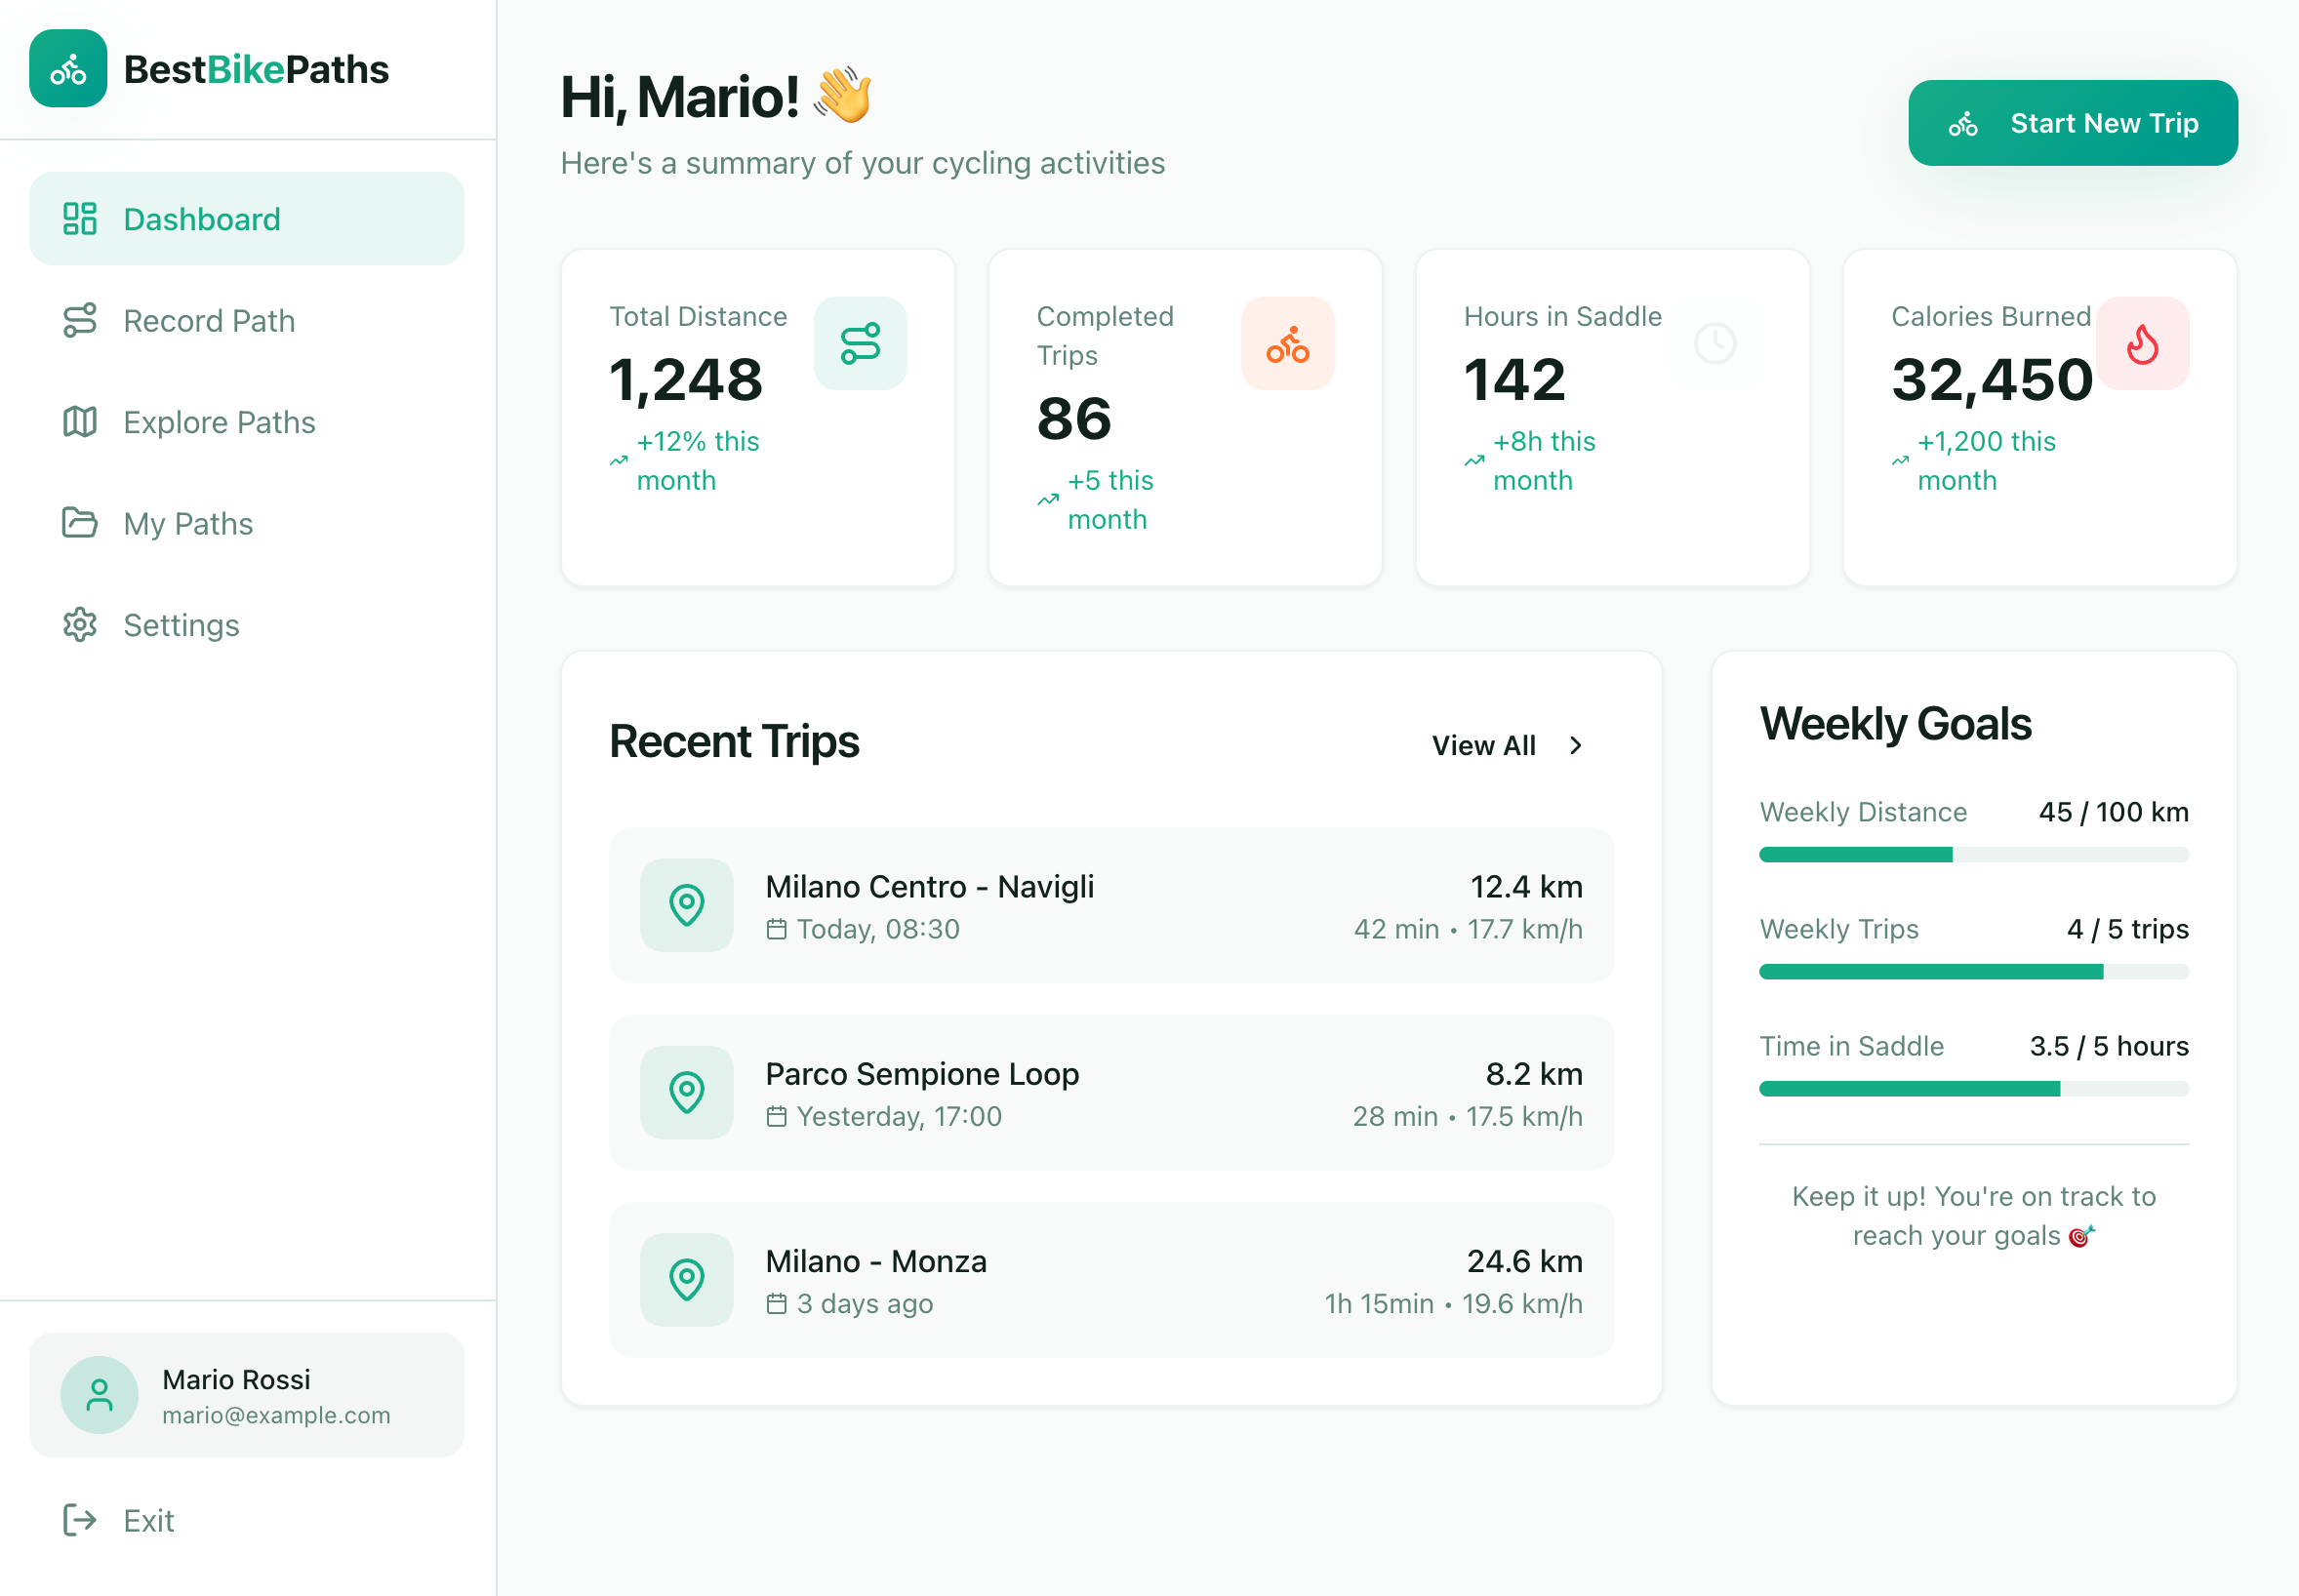
\includegraphics[width=0.8\textwidth]{Images/dashboard.png}
	\caption{Main dashboard summarizing service status, recent notifications, and quick actions.}
	\label{fig:dashboard}
\end{figure}

The \textbf{dashboard} provides an immediate summary of the most relevant information: \textbf{active services status}, \textbf{recent notifications}, \textbf{shortcuts} to the most frequent actions, and compact \textbf{trend charts}. Content is organized in \textbf{cards} to allow fast scanning and \textbf{responsive} flow; each card highlights the primary \textbf{KPI} or status and, when relevant, a \textbf{trend indicator}. A \textbf{left navigation bar} leads to the operational sections, while the \textbf{header} shows the name of the user and a button to \textbf{record a new activity}.

\begin{figure}[H]
	\centering
	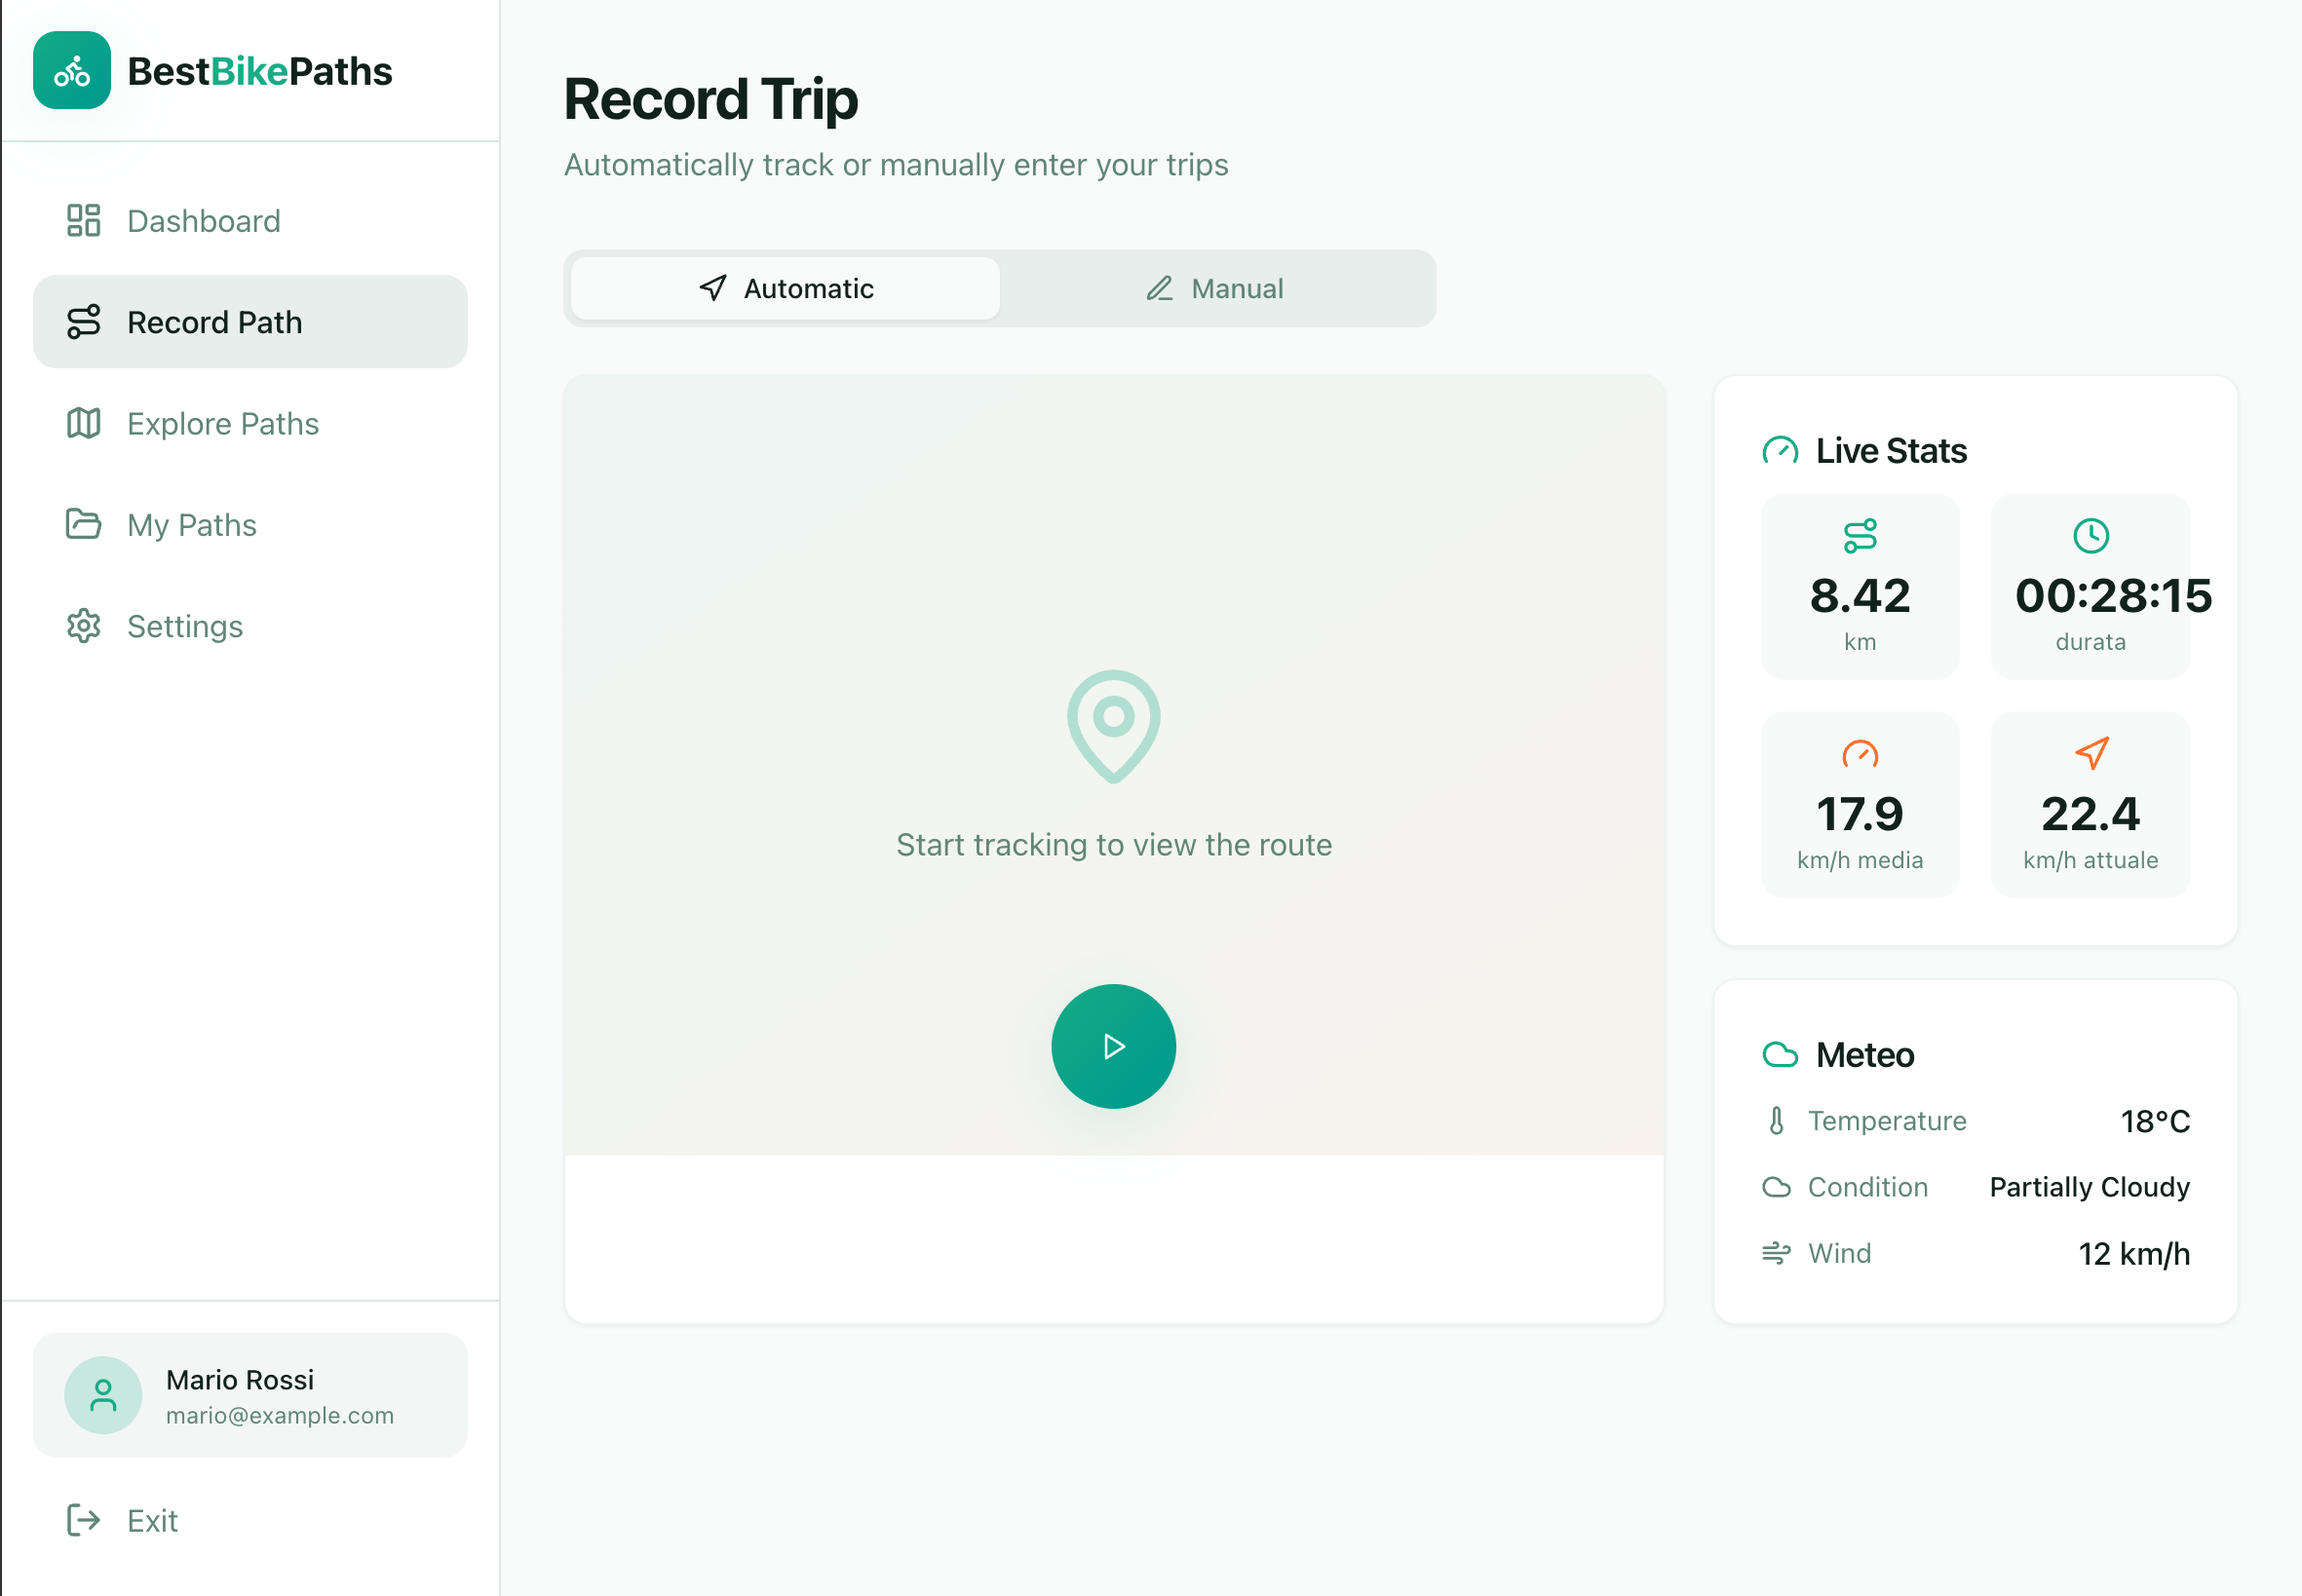
\includegraphics[width=0.8\textwidth]{Images/registra_viaggio.png}
	\caption{Trip recording interface with live metrics and waypoint controls.}
	\label{fig:registra-viaggio}
\end{figure}
The recording screen foregrounds the \textbf{start/stop control} and \textbf{live metrics} (\textbf{distance}, \textbf{duration}, \textbf{pace}). Secondary actions allow adding \textbf{waypoints} or \textbf{notes}; the layout keeps high \textbf{contrast} for outdoor readability.

\begin{figure}[H]
	\centering
	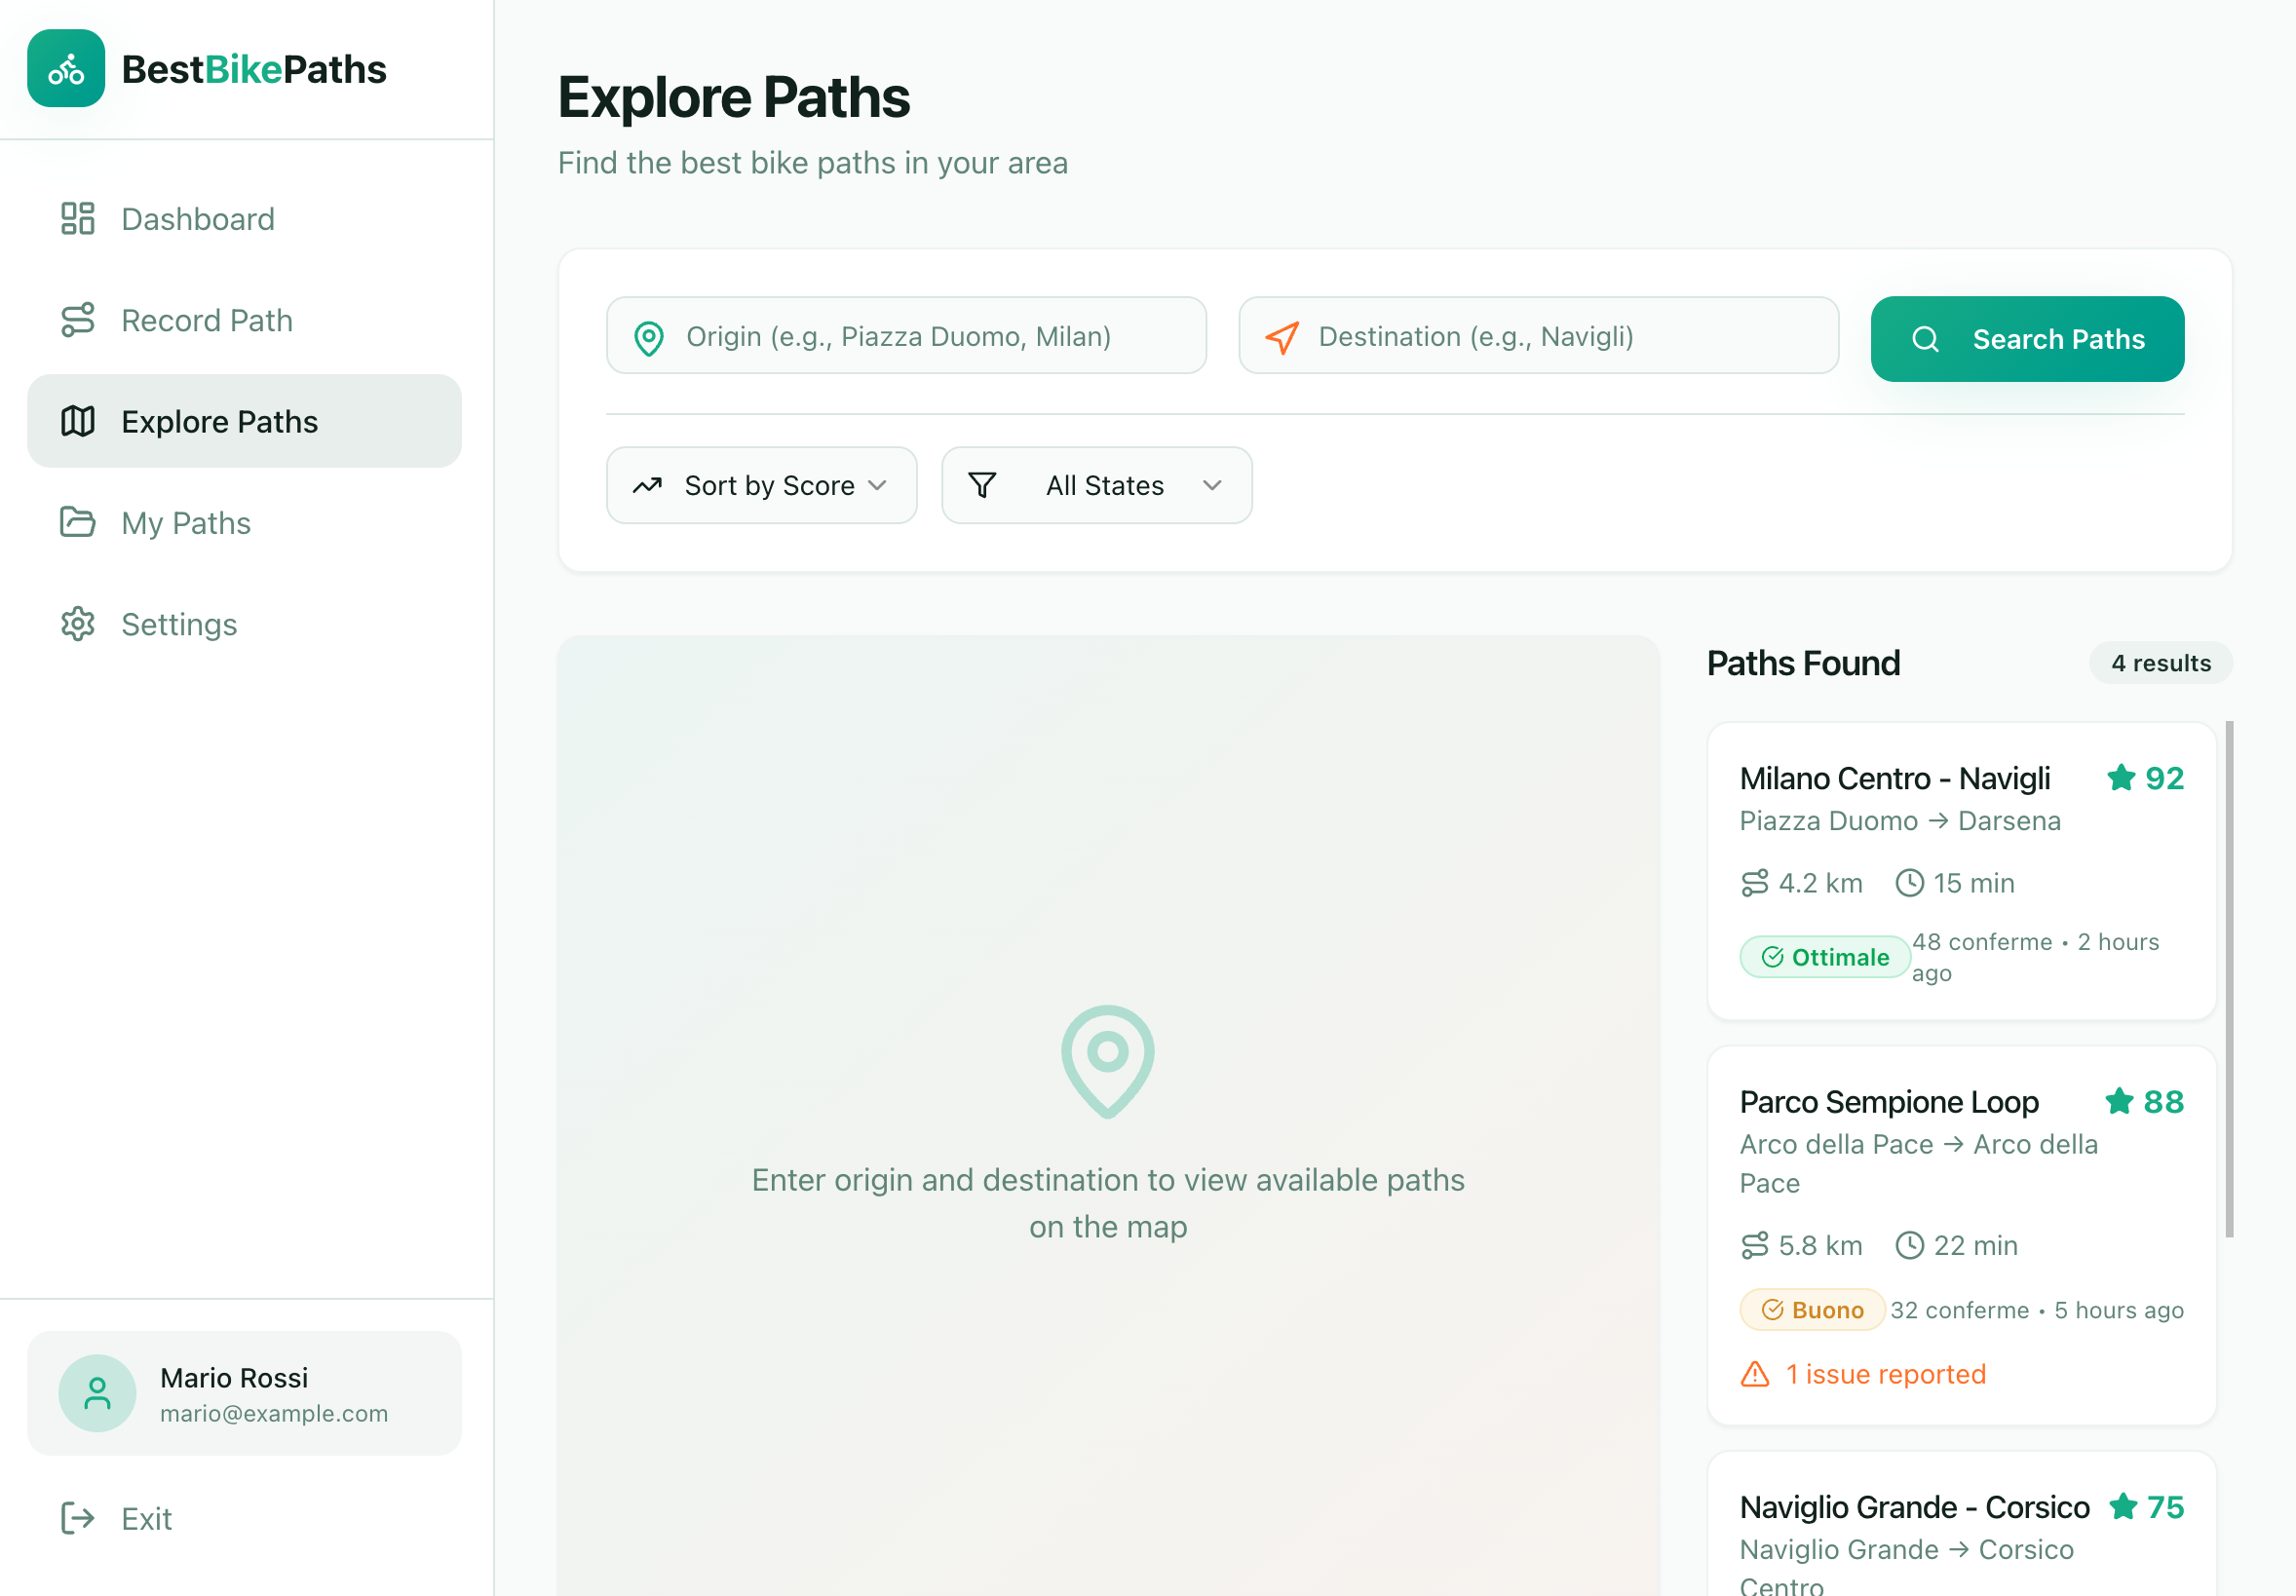
\includegraphics[width=0.8\textwidth]{Images/esplora_percorsi.png}
	\caption{Explore curated and suggested routes with filters and key stats.}
	\label{fig:esplora-percorsi}
\end{figure}
The explore view offers \textbf{curated and suggested routes} with \textbf{filters} for \textbf{difficulty}, \textbf{duration}, and \textbf{location}. Cards show a brief \textbf{description}, \textbf{tags}, and primary \textbf{stats} to help selection at a glance.

\begin{figure}[H]
	\centering
	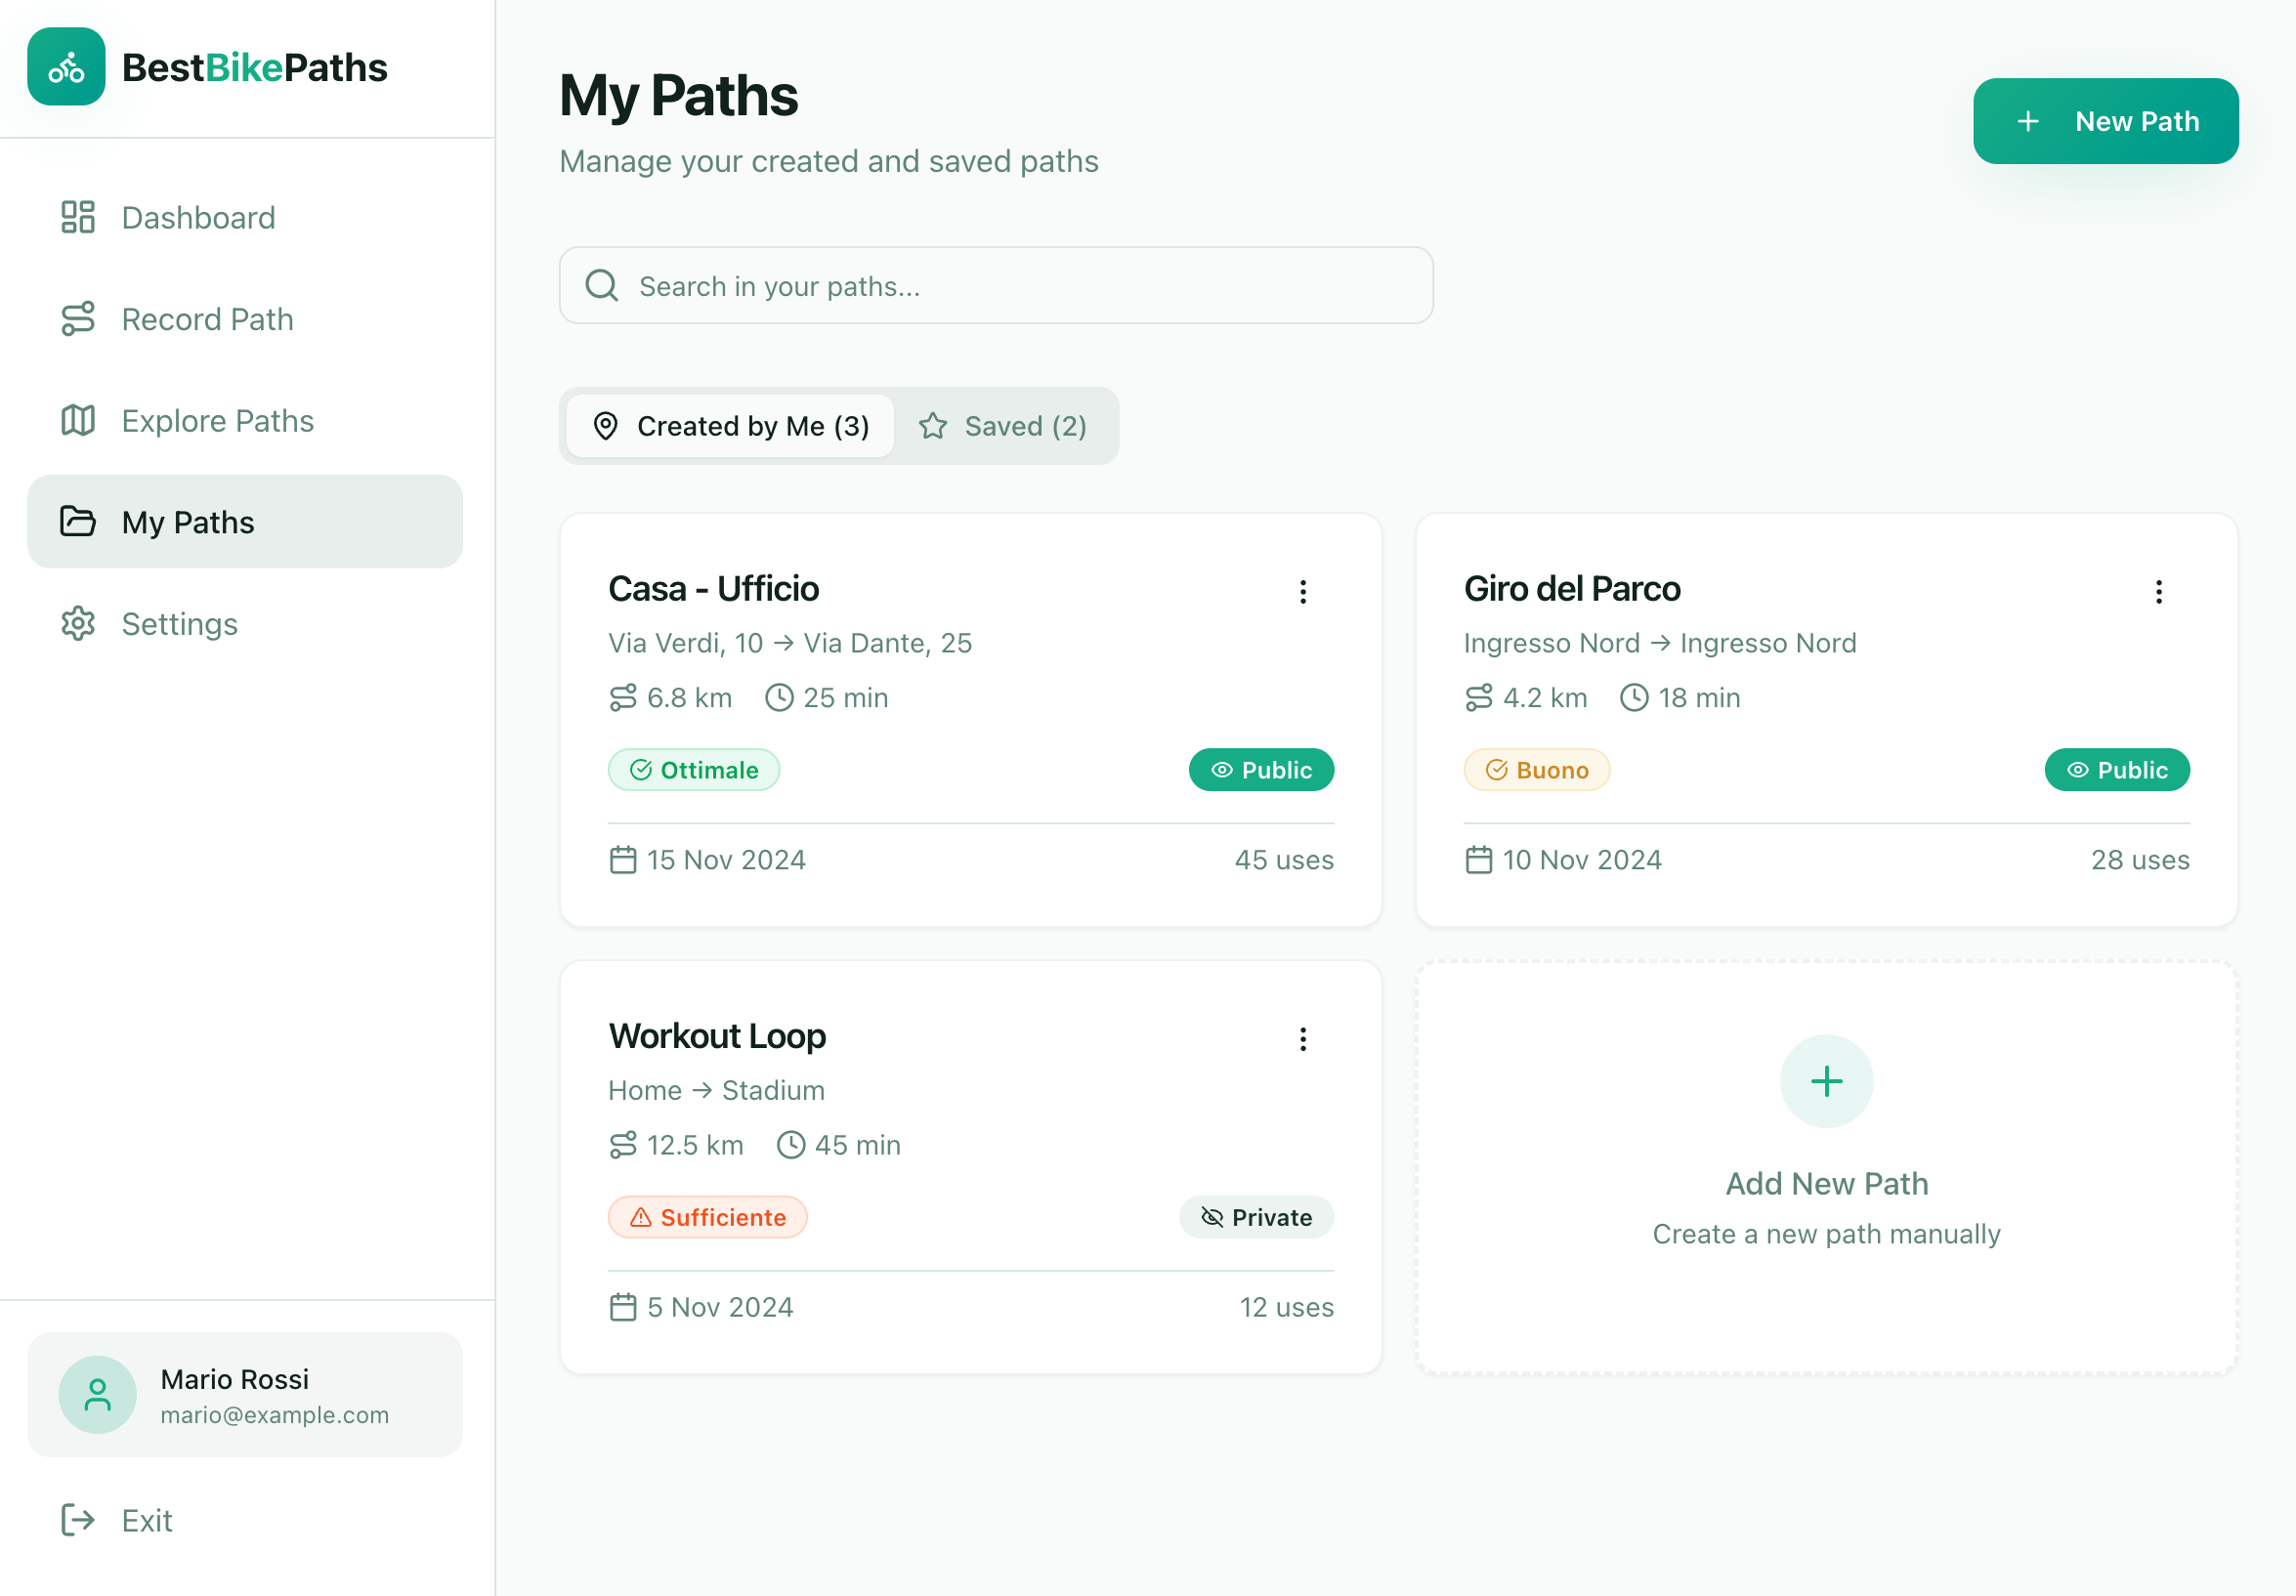
\includegraphics[width=0.8\textwidth]{Images/miei_percorsi.png}
	\caption{List of saved routes with quick access to details and navigation.}
	\label{fig:miei-percorsi}
\end{figure}

This screen lists the user \textbf{saved routes} with key \textbf{metadata} (\textbf{name}, \textbf{distance}, \textbf{duration}, \textbf{last update}) and quick entry points to view \textbf{details} or start \textbf{navigation}. Rows are designed for scannability and expose \textbf{status badges} for \textbf{drafts} or \textbf{shared items}.





\begin{figure}[H]
	\centering
	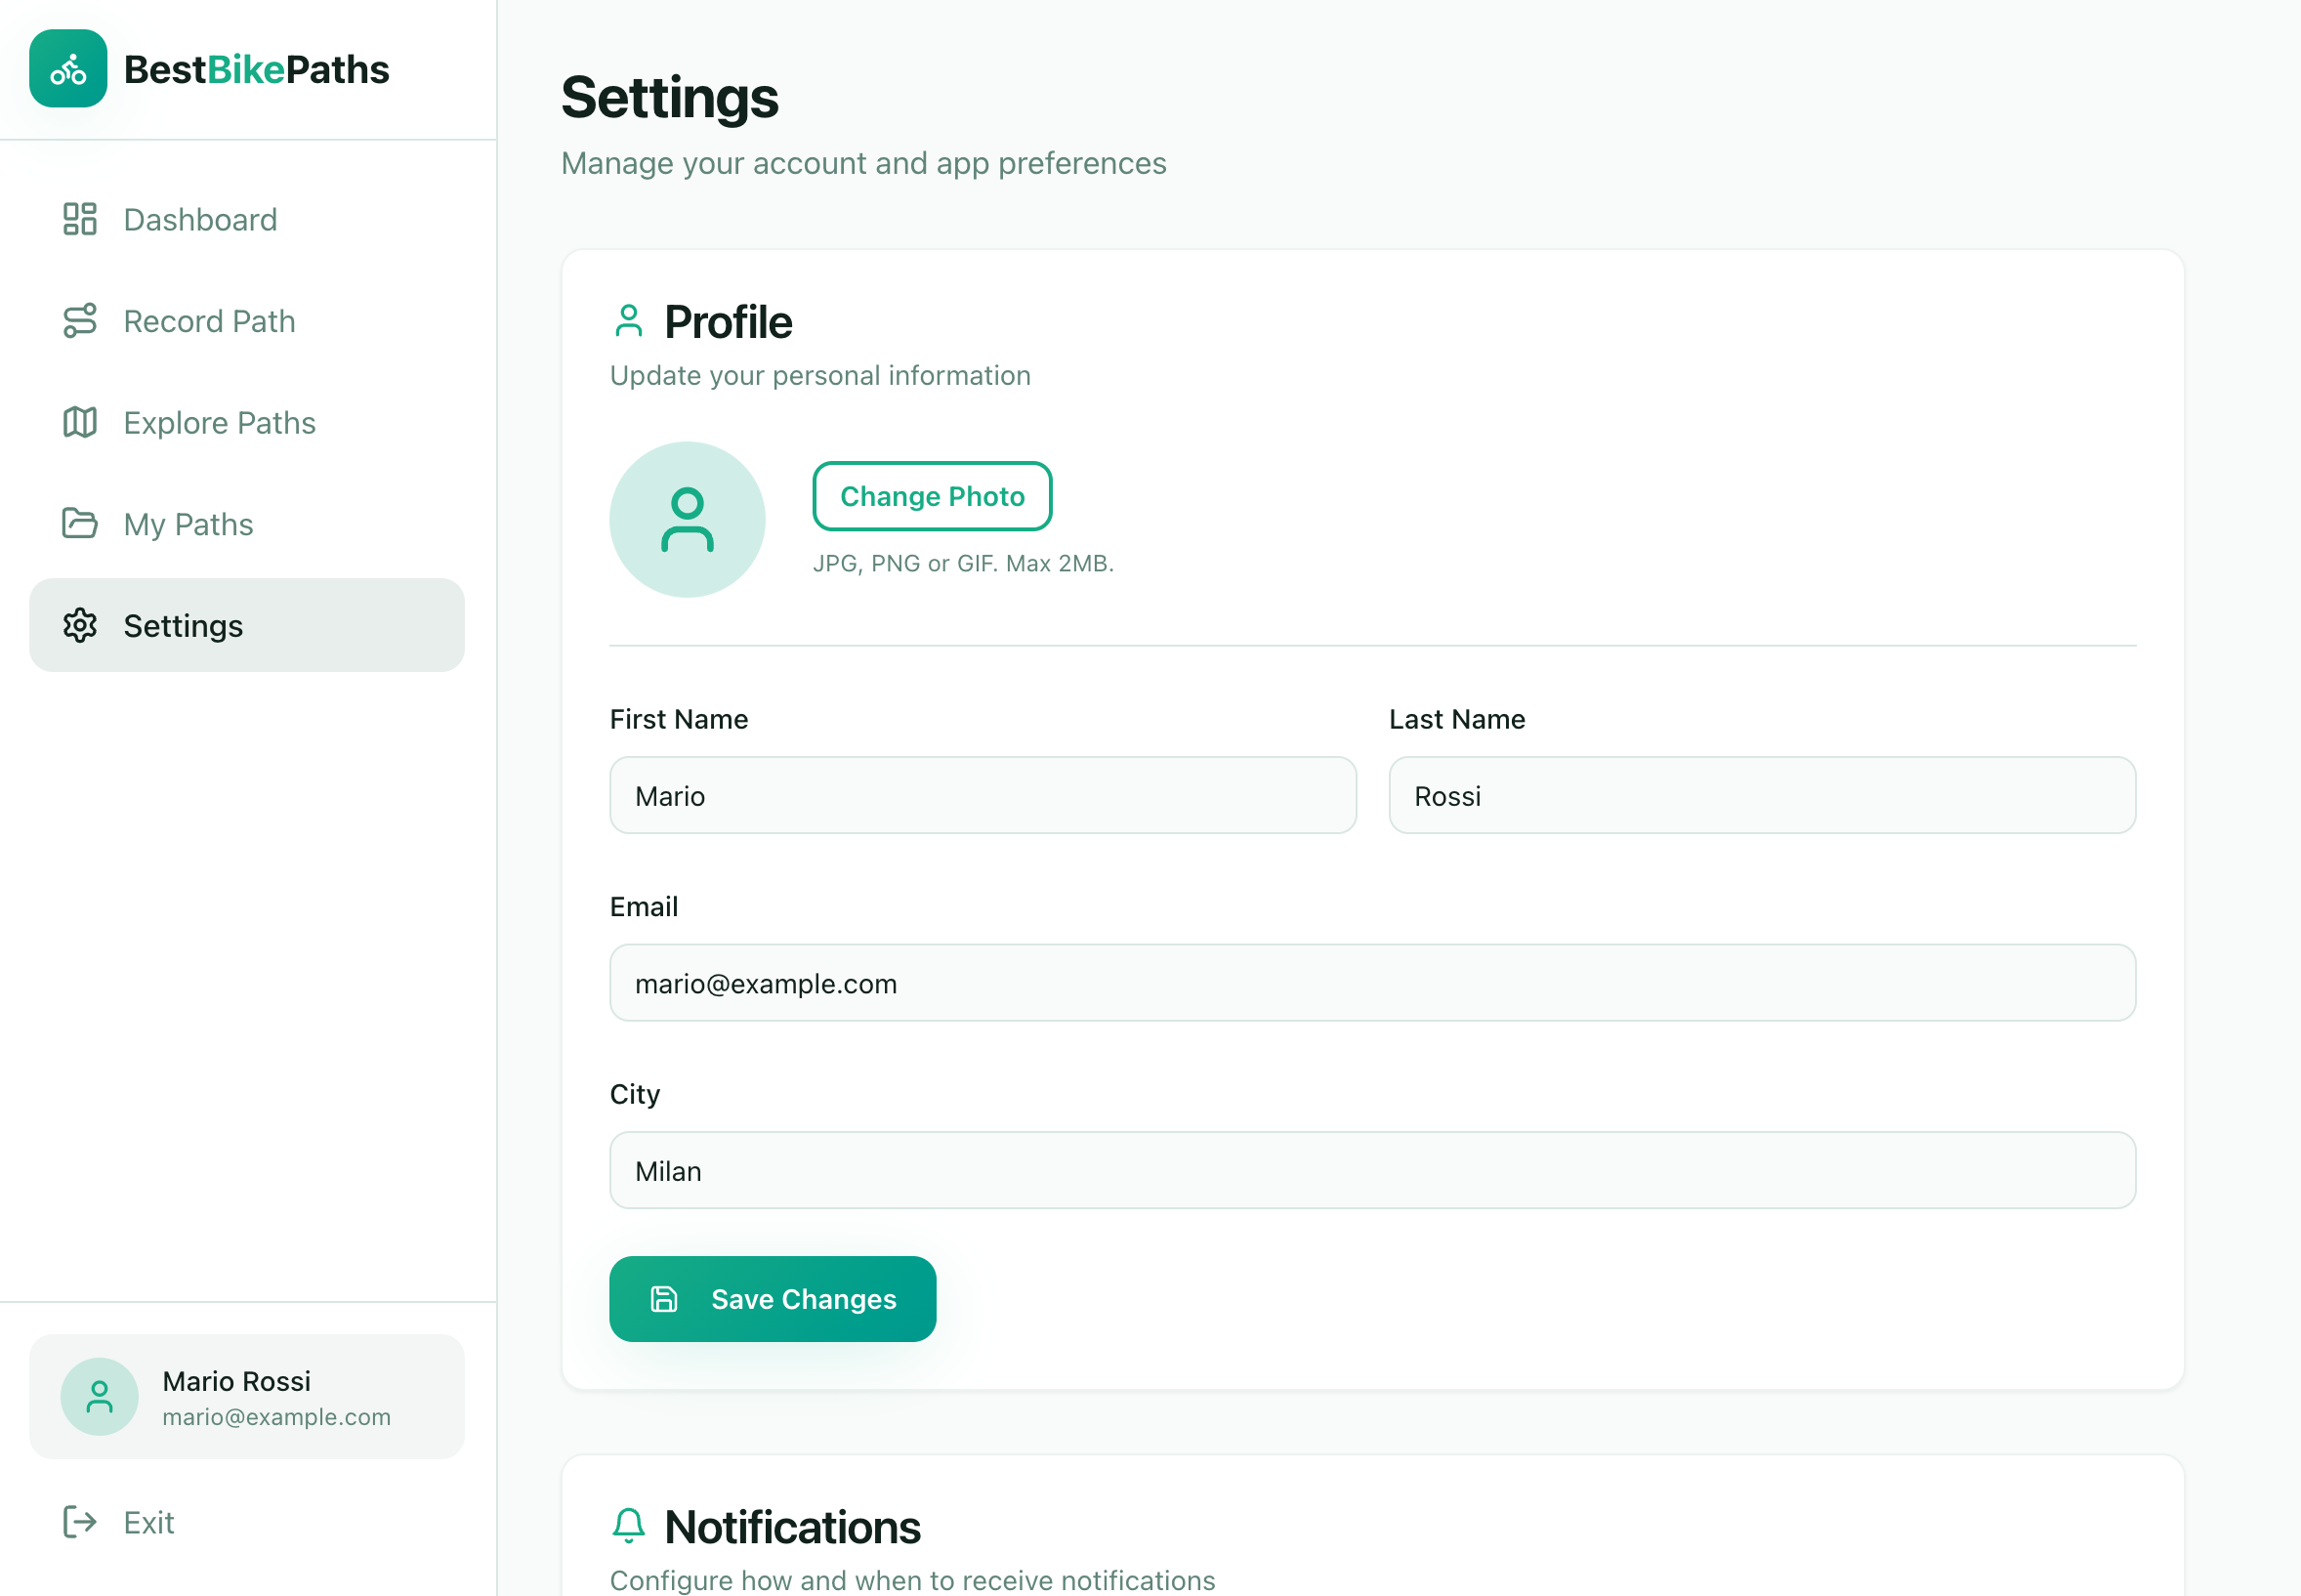
\includegraphics[width=0.8\textwidth]{Images/impostazioni.png}
	\caption{Settings grouped by account, privacy, and notifications.}
	\label{fig:impostazioni}
\end{figure}
Settings centralize \textbf{account}, \textbf{privacy}, and \textbf{notification preferences}. \textbf{Destructive actions} are visually separated.
